
\section{Add/Subtract Fractions}

In this lesson, we will learn how to add and subtract fractions.

\subsection{Add/Subtract Fractions with the Same Denominator}

We will do $\frac{1}{3}+\frac{1}{3}$ by graphing:

\begin{center}
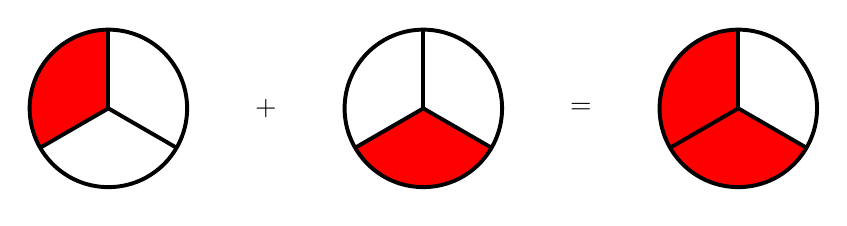
\begin{tikzpicture}
	\fill[red] (0,0) -- (0,1) arc (90:210:1cm) -- cycle;
	\draw[line width=0.5mm] (0,0) circle (1cm);
	\draw[line width=0.5mm] (0,0) -- (0,1);
	\draw[line width=0.5mm] (0,0) -- (0.8661,-0.5);
	\draw[line width=0.5mm] (0,0) -- (-0.8661,-0.5);
	
	\draw (2,0) node{+};
	
	\fill[red] (4,0) -- (-0.8661+4,-0.5) arc (210:330:1cm) -- cycle;
	\draw[line width=0.5mm] (4,0) circle (1cm);
	\draw[line width=0.5mm] (4,0) -- (4,1);
	\draw[line width=0.5mm] (4,0) -- (0.8661+4,-0.5);
	\draw[line width=0.5mm] (4,0) -- (-0.8661+4,-0.5);
	
	\draw (6,0) node{=};
	
	\fill[red] (8,0) -- (8,1) arc (90:210:1cm) -- cycle;
	\fill[red] (8,0) -- (-0.8661+8,-0.5) arc (210:330:1cm) -- cycle;
	\draw[line width=0.5mm] (8,0) circle (1cm);
	\draw[line width=0.5mm] (8,0) -- (8,1);
	\draw[line width=0.5mm] (8,0) -- (0.8661+8,-0.5);
	\draw[line width=0.5mm] (8,0) -- (-0.8661+8,-0.5);
	
\end{tikzpicture}
\captionof{figure}{$\frac{1}{3}+\frac{1}{3}=\frac{2}{3}$}
\end{center}

It's easy to see $\frac{1}{3}+\frac{1}{3}=\frac{2}{3}$. When we add fractions, we simply add the numerators, but the denominator doesn't change. The same rule applies when we subtract fractions.

\begin{myexample}
\[ 
\begin{aligned}[t]
	&\phantom{{}=}\frac{1}{5}+\frac{2}{5}+\frac{2}{5} \\
	&= \frac{1+2+2}{5} \\
	&= \frac{5}{5} \\
	&= 1
\end{aligned}
\]
\end{myexample}

\begin{myexample}
\[ 
\begin{aligned}[t]
	&\phantom{{}=}\frac{4}{5}-\frac{2}{5}+\frac{1}{5} \\
	&= \frac{4-2+1}{5} \\
	&= \frac{3}{5}
\end{aligned}
\]
\end{myexample}

\subsection{Add/Subtract Fractions with Different Denominator}
We will use $\frac{1}{2}+\frac{1}{4}$ as an example. First, we will do this in the "easy" way (wrong way):
\[ 
\begin{aligned}[t]
	&\phantom{{}=}\frac{1}{2}+\frac{1}{4} \\
	&=\frac{1+1}{2+4} \\
	&=\frac{2}{6} \\
	&=\frac{1}{3} 
\end{aligned}
\]

If we simply add the numerators and denominators, like what we did, it doesn't make sense. If we add up $\frac{1}{2}$ and $\frac{1}{4}$, the answer cannot be $\frac{1}{3}$, because $\frac{1}{3}$ is smaller than $\frac{1}{2}$. We must change the denominators to the same number, before adding up the numerators.

Earlier, we learned how to find the LCM (Least Common Multiple) of a group of numbers. This is a good opportunity to go back and review that lesson.

Since $2$ goes into $4$, the LCM of $2$ and $4$ is simply $4$. To change $\frac{1}{2}$ to $\frac{?}{4}$, we multiply $2$ in both the numerator and denominator of $\frac{1}{2}$. The full solution is:
\[ 
\begin{aligned}[t]
	&\phantom{{}=}\frac{1}{2}+\frac{1}{4} \\
	&=\frac{1\cdot2}{2\cdot2}+\frac{1}{4} \\
	&=\frac{2}{4}+\frac{1}{4} \\
	&=\frac{2+1}{4} \\
	&=\frac{3}{4} 
\end{aligned}
\]
This result makes sense because half a dollar (50 cents) plus a quarter (25 cents) is three quarters (75 cents). Let's understand this problem by graph:

\begin{center}

\begin{tikzpicture}
	\fill[red] (0,0) -- (0,1) arc (90:270:1cm) -- cycle;
	\draw[line width=0.5mm] (0,0) circle (1cm);
	\draw[line width=0.5mm] (0,-1) -- (0,1);
	
	\draw (1.5,0) node{+};
	
	\fill[red] (0+3,0) -- (0+3,1) arc (90:0:1cm) -- cycle;
	\draw[line width=0.5mm] (0+3,0) circle (1cm);
	\draw[line width=0.5mm] (-1+3,0) -- (1+3,0);
	\draw[line width=0.5mm] (0+3,-1) -- (0+3,1);
	
	\draw (4.5,0) node{=};
	
	\fill[red] (0+6,0) -- (0+6,1) arc (90:270:1cm) -- cycle;
	\draw[line width=0.5mm] (0+6,0) circle (1cm);
	\draw[line width=0.5mm] (-1+6,0) -- (1+6,0);
	\draw[line width=0.5mm] (0+6,-1) -- (0+6,1);
	
	\draw (7.5,0) node{+};
	
	\fill[red] (0+9,0) -- (0+9,1) arc (90:0:1cm) -- cycle;
	\draw[line width=0.5mm] (0+9,0) circle (1cm);
	\draw[line width=0.5mm] (-1+9,0) -- (1+9,0);
	\draw[line width=0.5mm] (0+9,-1) -- (0+9,1);
	
	\draw (10.5,0) node{=};
	
	\fill[red] (0+12,0) -- (0+12,1) arc (90:270:1cm) -- cycle;
	\fill[red] (0+12,0) -- (0+12,1) arc (90:0:1cm) -- cycle;
	\draw[line width=0.5mm] (0+12,0) circle (1cm);
	\draw[line width=0.5mm] (-1+12,0) -- (1+12,0);
	\draw[line width=0.5mm] (0+12,-1) -- (0+12,1);
	
\end{tikzpicture}
\captionof{figure}{$\frac{1}{2}+\frac{1}{4}=\frac{3}{4}$}
\end{center}

In the graph, the first step is to cut $\frac{1}{2}$ into twice as many pieces, which changes $\frac{1}{2}$ into $\frac{2}{4}$. Understand that when we do $\frac{1}{2}=\frac{1\cdot2}{2\cdot2}=\frac{2}{4}$, we are simply cutting the whole into more pieces without changing the fraction's value.

The rule is the same when we subtract fractions with different denominators.

\begin{myexample}
\[ 
\begin{aligned}[t]
	&\phantom{{}=}\frac{1}{2}-\frac{1}{3} \\
	&=\frac{1\cdot3}{2\cdot3}-\frac{1\cdot2}{3\cdot2} \\
	&=\frac{3}{6}-\frac{2}{6} \\
	&=\frac{3-2}{6} \\
	&=\frac{1}{6} 
\end{aligned}
\]
The LCM of $2$ and $3$ is $6$.
\end{myexample}

If the answer can be reduced, we must do so, as in the next example.

\begin{myexample}
\[ 
\begin{aligned}[t]
	&\phantom{{}=}\frac{1}{2}-\frac{1}{6} \\
	&=\frac{1\cdot3}{2\cdot3}-\frac{1}{6} \\
	&=\frac{3}{6}-\frac{1}{6} \\
	&=\frac{3-1}{6} \\
	&=\frac{2}{6} \\
	&=\frac{2\div2}{6\div2} \\
	&=\frac{1}{3} 
\end{aligned}
\]
In the last step, we must reduce $\frac{2}{6}$ to $\frac{1}{3}$. Make it a habit to check whether a fraction can be reduced. Try the first few prime numbers: $2,3,5,7,11$.
\end{myexample}

\subsection{Fraction Word Problems}
\begin{myexample}
Omar and Jose are painting a room. Omar can paint the whole room in $8$ hours if he works by himself, while Jose can paint the whole room in $4$ hours. If they work together, what fraction of the job can be done in one hour?
\end{myexample}
\begin{solution}
Since Omar can paint the whole room in $8$ hours, he can complete $\frac{1}{8}$ of the job in one hour.

Similarly, Jose can complete $\frac{1}{4}$ of the job in one hour.

To find what fraction of the job can be done if they work together, we add up the fraction of the job each person can complete:
\[ 
\begin{aligned}[t]
	&\phantom{{}=}\frac{1}{8}+\frac{1}{4} \\
	&=\frac{1}{8}+\frac{1\cdot2}{4\cdot2} \\
	&=\frac{1}{8}+\frac{2}{8} \\
	&=\frac{1+2}{8} \\
	&=\frac{3}{8} 
\end{aligned}
\]
If they work together, $\frac{3}{8}$ of the job can be done in one hour.
\end{solution}

\begin{myexample}
Tom, Jerry and Peter are sharing a pizza. Tom ate $\frac{2}{5}$ of the pizza; Jerry ate $\frac{1}{4}$ of the pizza; Peter ate the rest. What fraction of the pizza did Peter eat?
\end{myexample}
\begin{solution}
The whole pizza is a whole $1$. After Tom ate $\frac{2}{5}$ and Jerry ate $\frac{1}{4}$, what's left is:
\[ 
\begin{aligned}[t]
	&\phantom{{}=}1-\frac{2}{5}-\frac{1}{4} \\
	&=\frac{1}{1}-\frac{2}{5}-\frac{1}{4} \\
	&=\frac{1\cdot20}{1\cdot20}-\frac{2\cdot4}{5\cdot4}-\frac{1\cdot5}{4\cdot5} \\
	&=\frac{20}{20}-\frac{8}{20}-\frac{5}{20} \\
	&=\frac{7}{20} \\
\end{aligned}
\]
Peter ate $\frac{7}{20}$ of the pizza.

Note that the LCM of $1$, $5$ and $4$ is $20$.
\end{solution}

\subsection{Summary}
Let's review what we learned in this lesson:
\begin{itemize}
\item To add/subtract fractions with the same denominator, we add/subtract the numerators, and keep the denominator unchanged. For example: 
\[ \frac{3}{5}+\frac{1}{5}=\frac{3+1}{5}=\frac{4}{5} \]
\item To add/subtract fractions with different denominators, first change the denominator to the same number (their LCM), and then add/subtract the numerators. For example: 
\[ \frac{1}{2}+\frac{1}{3}=\frac{1\cdot3}{2\cdot3}+\frac{1\cdot2}{3\cdot2}=\frac{3}{6}+\frac{2}{6}=\frac{3+2}{6}=\frac{5}{6} \]
\end{itemize}

